% A gépnyilvántartás adatmodellje (5. fejezet). Fordítás: pdflatex adatmodell.tex
\documentclass[tikz,border=4pt]{standalone}
\usepackage[utf8]{inputenc}
\usepackage[T1]{fontenc}
\usepackage{times}
\usetikzlibrary{positioning,arrows.meta,shapes.multipart}
\definecolor{det}{HTML}{1D294D}
\definecolor{detbg}{HTML}{E6ECF7}
\begin{document}
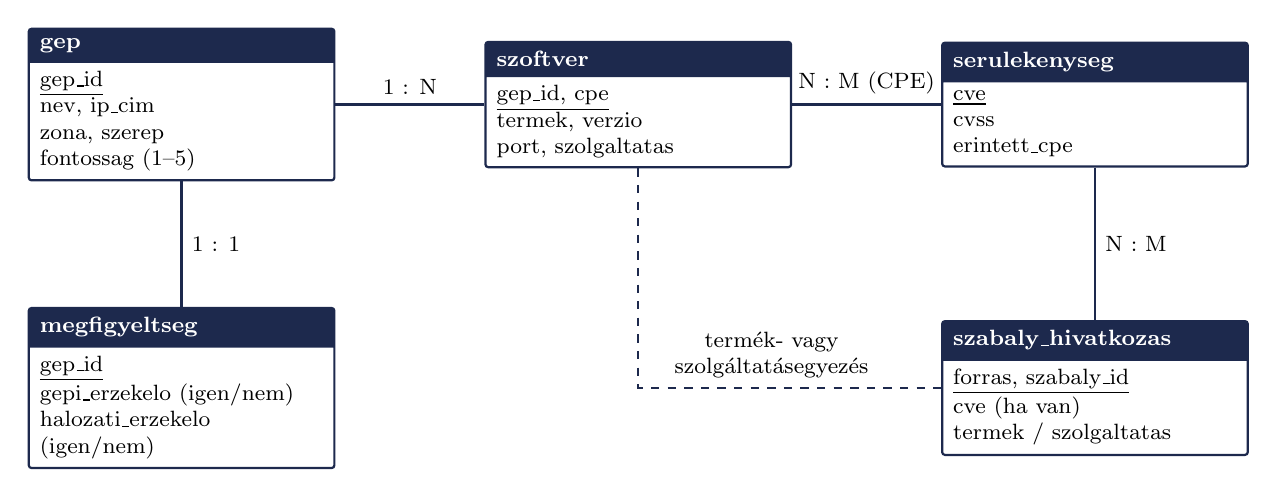
\begin{tikzpicture}[
  font=\footnotesize,
  tbl/.style={rectangle split, rectangle split parts=2, draw=det, thick, rounded corners=1pt,
              rectangle split part fill={det,white}, align=left, text width=36mm,
              inner xsep=4pt, inner ysep=3pt},
  rel/.style={thick, draw=det},
]
\newcommand{\tname}[1]{\textcolor{white}{\textbf{#1}}}
\node[tbl] (gep) at (0,0) {\tname{gep}\nodepart{two}%
  \underline{gep\_id}\\ nev, ip\_cim\\ zona, szerep\\ fontossag (1--5)};
\node[tbl] (megf) at (0,-36mm) {\tname{megfigyeltseg}\nodepart{two}%
  \underline{gep\_id}\\ gepi\_erzekelo (igen/nem)\\ halozati\_erzekelo (igen/nem)};
\node[tbl] (szolg) at (58mm,0) {\tname{szoftver}\nodepart{two}%
  \underline{gep\_id, cpe}\\ termek, verzio\\ port, szolgaltatas};
\node[tbl] (cve) at (116mm,0) {\tname{serulekenyseg}\nodepart{two}%
  \underline{cve}\\ cvss\\ erintett\_cpe};
\node[tbl] (szab) at (116mm,-36mm) {\tname{szabaly\_hivatkozas}\nodepart{two}%
  \underline{forras, szabaly\_id}\\ cve (ha van)\\ termek / szolgaltatas};
\draw[rel] (gep.east) -- node[above]{1 : N} (szolg.west);
\draw[rel] (szolg.east) -- node[above]{N : M (CPE)} (cve.west);
\draw[rel] (gep.south) -- node[right]{1 : 1} (megf.north);
\draw[rel] (cve.south) -- node[right]{N : M} (szab.north);
\draw[rel, dashed] (szolg.south) |- node[pos=0.72, above, align=center]{termék- vagy\\ szolgáltatásegyezés} (szab.west);
\end{tikzpicture}
\end{document}
